\chapter{Studies of environmental noise during O3}

{\color{red}
Introduce how observing/engineering runs work, O3 schedule, etc.}

\ac{O3} was preceded by an engineering run, a month-long period during with the interferometer is operational at low-noise levels but not observing \ac{GW} events, to provide time for detector commissioning and noise studies.

\section{Vibrational noise studies during O3}\label{sec:noise-vib}

\begin{figure}[h!]
	\centering
	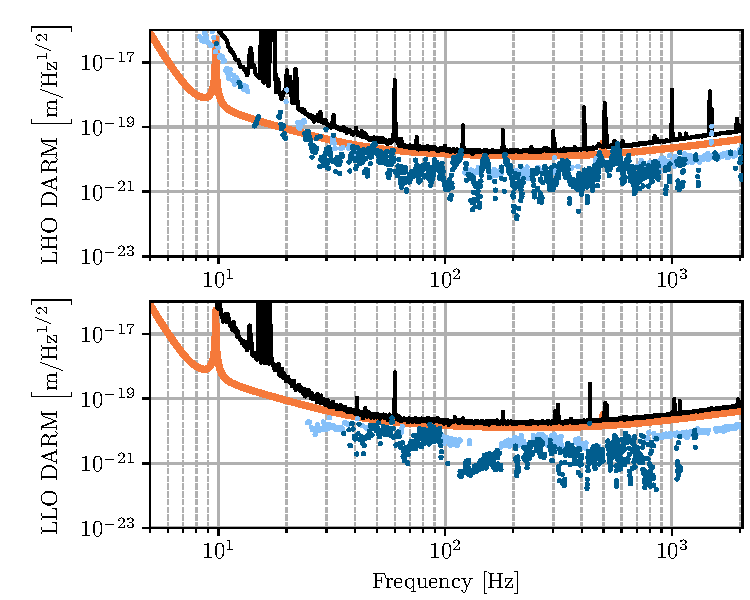
\includegraphics[width=\textwidth]{figures/ambient_vib.pdf}
	\caption{
		Ambient estimate of vibrational noise levels at LHO (top) and LLO (bottom).}
	\label{fig:ambient-vib}
\end{figure}

Figure~\ref{fig:ambient-vib} shows the ambient contribution of vibrational noise during \ac{O3}, produced by combining the highest coupling factors among accelerometers and microphones measured from an injection campaign at the beginning of \ac{O3}.
At the end of \ac{O3}, the vibration noise background at both observatories was dominated by input beam jitter above 100\,Hz (discussed in Section~\ref{sec:jitter}).
At \ac{LHO},  the dominant coupling region below 100\,Hz was the output arm.
At \ac{LLO}, the dominant coupling regions were the Y-end in the 40-60\,Hz band and the output arm in the 60-100\,Hz band.

\subsection{Scattered light at the HAM5/6 septum}\label{sec:noise-vib-scatter}

A major source of detector noise and reduced sensitivity to \acp{GW} is the scattering of light from the beam spot on a test mass or other optic to surfaces that are moving relative to the optic, like vacuum chamber walls.
A very small fraction of the light reaching the moving surface is reflected to the originating or another beam spot, where it scatters back into the main interferometer beam.
As the distance to the moving surface changes, the phase of the returning light changes relative to the main beam, producing fluctuations in the amplitude of the beam, that, at 1 part in $10^{20}$ can be on the scale of those produced by gravitational waves.
In addition to this sensitivity to recombined scattered light, the scattering noise is problematic because of non-linear coupling when the path length modulation becomes comparable to the wavelength of the light, producing noise at harmonics of modulation frequencies~\citep{Soni_2020}.

At \ac{LHO}, investigations throughout \ac{O3} showed that scattering noise produces noise near the detector noise background in the frequency range of 38--100\,Hz.
The sensors with the highest ambient projections in this band were accelerometers located on the HAM 5 and HAM 6 vacuum chambers, which contain the \ac{GW} channel readout, as well as the optics of the output mode cleaner, squeezed light system, and signal recycling cavity.
The coupling was excited most strongly by injections around the output arm, but acoustic noise produced as far as the Y-arm manifold $\approx 50$\,m away produced excess noise in \ac{DARM}.


\subsection{Search for the source of a 48-Hz peak}\label{sec:noise-vib-48hz}

{\color{red}
To-do.}

\begin{figure}
	\centering
	\includegraphics[width=\textwidth]{figures/48Hz.png}
	\caption{LHO DARM spectrum before and after mitigation of the 48-Hz peak.}
	\label{fig:48hz}
\end{figure}

\subsection{Input beam jitter}\label{sec:noise-vib-jitter}

{\color{red}
Short discussion, summarize measurements and improvement.
Will make sure to discuss impact of test mass defect on jitter noise.}

\begin{figure}
	\centering
%	\includegraphics[width=\textwidth]{}
	\caption{Improvement in jitter coupling at LHO (left) and LLO (right) between the start and end of O3.}
	\label{fig:jitter}
\end{figure}

\section{Magnetic noise studies during O3}\label{sec:noise-mag}

\begin{figure}[h]
	\centering
	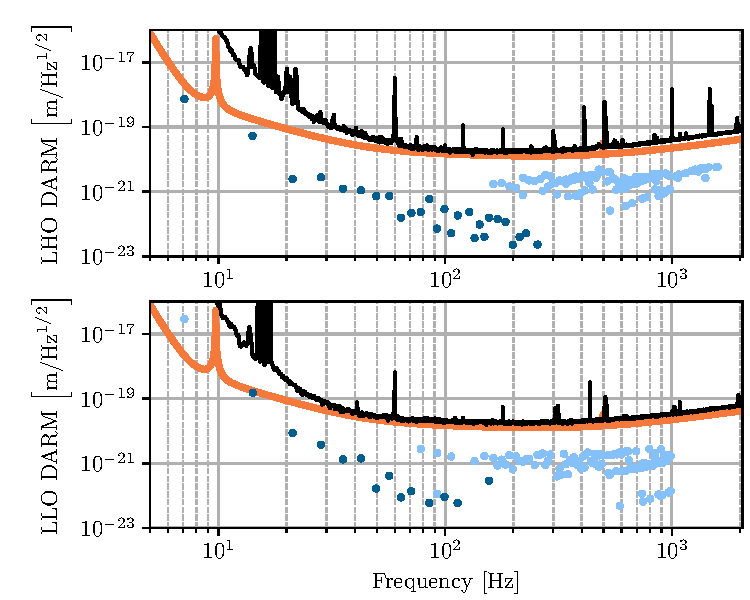
\includegraphics[width=\textwidth]{figures/ambient_mag.pdf}
	\caption{
		Ambient estimate of magnetic noise levels at LHO (top) and LLO (bottom).}
	\label{fig:ambient-mag}
\end{figure}

Magnetic injections early in \ac{aLIGO} suggested that coupling to permanent magnets in the suspension system  could prevent \ac{LIGO} from reaching design sensitivity in the 10-20\,Hz regions~\citep{Schofield_2013}.
While the test mass actuator is electrostatic and not magnetic (as in \ac{iLIGO}), a number of permanent magnets were used in the suspensions, including for actuation in the first three of the four levels of the isolation chain and for eddy current damping.
The greatest number of permanent magnets were in the eddy current damping arrays and these were removed.
Nevertheless, ambient fields are still predicted to produce noise at greater than one-tenth of the design sensitivity in the 10-20\,Hz band (Figure~\ref{fig:ambient-mag}), and may need to be further addressed as we reach design sensitivity in the 10\,Hz region.

At higher frequencies, generally above about 30\,Hz, the dominant magnetic coupling appears to be through induction of currents in cables and at connectors, mainly to actuator cabling and other cabling in the control system.
Mitigation of coupling to cables and connectors has required a continuing program of monitoring coupling since cables are often disconnected and reconnected during runs as electronics are replaced for problems or upgrades.
This program consists of making weekly, broadband magnetic field injections using the large wall-mounted coils described in Section~\ref{sec:magnetic-injections}.
The injections have shown that peaks can appear or disappear, as well as shift in frequency, on a weekly basis.

\subsection{Fluctuations in magnetic coupling}\label{sec:noise-mag-weekly}

\begin{figure}
	\centering
%	\includegraphics[width=\textwidth]{}
	\caption{
		Ambient estimate of magnetic noise levels at LHO on Mar \XX, 2019 (blue), \XX weeks before O3, and on Apr \XX, 2019 (orange), \XX weeks into O3.}
	\label{fig:weekly-mag-preO3}
\end{figure}

\begin{figure}
	\centering
%	\includegraphics[width=\textwidth]{}
	\caption{Weekly trends in frequency (top) and amplitude (top) of peaks in the magnetic coupling functions.}
	\label{fig:weekly-mag-variation}
\end{figure}

\section{Validation of gravitational wave event candidates}\label{subsec:vetting}

In addition to investigating sources of environmental influences, knowledge acquired from environmental studies contributes to the vetting of \ac{GW} event candidates.
Analysis pipelines search the strain data for astrophysical signals.
They are categorized into modeled searches for binary mergers that match the data to template waveforms (e.g. GstLAL~\citep{Cannon_2012} and PyCBC~\citep{Usman_2016}) and un-modeled searches that identify excess energy coherent between multiple detectors (e.g. cWB~\citep{Klimenko_2008}, oLIB~\citep{Lynch_2017}, and BW~\citep{Cornish_2015}).

Contamination of the \ac{GW} data can occur through any of the means discussed in previous sections.
Environmental noise has the potential to be correlated between detectors by stemming from a common source, such as through electromagnetic signals from distant sources or glitches in GPS-correlated electronics.
The analysis pipelines estimate the false-alarm probabilities for GW events based on the background rate of randomly coincident events in the detector network.
They generate background events by time-shifting the data stream of one detector relative to another by time steps much longer than the light travel time between detectors and longer than the duration of GW signals.%~\citep{Was_2009}.
This method does not account for the possibility of transients being correlated between the detectors due to a common environmental source.

Environmental noise is also particularly relevant to un-modeled searches. Unlike template-based methods, these searches make minimal assumptions about the signal waveform and rely more heavily on signal correlation between sites.

The first observation of a \ac{GW} occurred on 14 Sept 2015~\citep{gw150914}.
The event, a short-duration binary black hole merger designated GW150914, required a number of follow-up investigations to find potential noise sources around the time of the event~\citep{Detchar_2016}.
This included an examination of the status of all \ac{PEM} sensors and any significant signals they observed for possible contamination of the GW signal~\citep{Schofield_150914}.
A few of the \ac{PEM} sensors were not working, but because of redundancy, coverage was sufficient.

Comparisons between Q-transform spectrograms~\citep{Chatterji_2004} of all coincident events in environmental sensors to the time-frequency path of the event revealed that no environmental signals had paths similar to the event candidate.
Q-transforms produce a quality-factor-optimized logarithmic tiling of the time-frequency space, making them useful for visualizing transients.
The \acp{SNR} of the matching signals were also compared to that of the event, showing that even if there were overlapping time-frequency paths, none of the environmental signals were large enough to influence the strain data at the \ac{SNR} level of the event, based on multiplying the environmental signals by their respective sensor coupling functions.

The validation process for novel events such as GW150914 also includes redundant checks for global sources of environmental noise.
We use a dedicated cosmic ray detector located below an input test mass at \ac{LHO} to examine any association of cosmic ray showers to excess noise in \ac{DARM}.
We also check external observatories for coronal mass ejections, solar radio signals, geomagnetic signals, and \ac{RF} signals in the detection band as well as higher frequencies.

There was specific concern over a co-incident extremely-high current (504\,kA) lightning strike over Burkina Faso, prompting additional studies of the effects of lightning on the interferometer~\citep{Schofield_lightning}.
Investigations of similar strikes found no effect on the strain data and investigations of closer strikes confirmed that the magnetometers were much more sensitive to lightning strikes than the interferometer was.
In conclusion there was no reason to veto the first detection based on environmental disturbances.

Subsequent detections throughout \ac{O1} and \ac{O2} employed a similar procedure; however the development of the method described in Section~\ref{sec:cf} for producing coupling functions for all sensors expedited the process.
This was especially important for examining environmental noise during GW170817, the first long-duration event detected by \ac{LIGO}~\citep{gw170817, Schofield_170817}.
The longer duration of this event (75\,s) unsurprisingly overlapped with many environmental signals.
Based on the coupling functions for those sensors, several of these environmental events were loud enough (estimated \ac{DARM} signals of up to SNR~4) to have contributed to the interferometer readout, but not enough to account for the \ac{GW} signal.
Furthermore, none of them had a time-frequency morphology that correlated with any features in the candidate signal.

Since \ac{O3}, most of the procedure described above has been automated in order to handle the increase in detection rate.
The automated vetting is performed by the \code{pemcheck} routine, which is a part of the \ac{DQR}.
When an event is detected by the astrophysical search pipelines, a \ac{DQR} is initiated and assembles a plethora of tasks for assessing the data quality at each observatory during the time of the event.
Among these tasks, an omega scan pipeline~\citep{Davis_2021, Chatterji_2004} is used to search for transient noise in all \ac{PEM} sensors in the time window spanning the event candidate.
It does so by producing a Q-transform for each sensor and reporting those in which there is a transient signal with a false-alarm rate below $10^{-3}$\,Hz.
The omega scan also reports the frequency and amplitude of the most significant tile for each sensor.
The \code{pemcheck} uses the output of the omega scan to estimate each sensor's potential affect on the data quality of the detector.
The coupling function of each sensor is interpolated at the peak frequency and multiplied by the peak amplitude, producing an estimated \ac{DARM} amplitude.

Sensors whose estimated contribution exceed one tenth of the \ac{DARM} background level are flagged for human input, requiring a comparison of the environmental signal morphology to that of the event candidate.
If there is sufficient signal overlap, reviewers may advise that analysts perform some noise removal in the data, such as by gating or filtering out the appropriate time or frequency range, before performing further follow up analyses.
The event could be retracted, if gating or filtering out the environmental contribution would reduce the signal-to-noise ratio of the candidate to a level no longer consistent with a GW detection.

During \ac{O3}, no candidates were retracted on the basis of the environmental coupling check alone.
Some human input was still required for all of the \XX events reported in~\citep{gwtc2}, although little to no signal overlap of environmental transients was seen.

{\color{red}
Discuss new pemcheck method.}
